\documentclass[aspectratio=169, 10pt]{beamer}

% ── Theme & Colors ────────────────────────────────────────────
\usetheme{metropolis}
\usepackage{appendixnumberbeamer}
\usepackage{booktabs}
\usepackage{graphicx}
\usepackage{xcolor}
\usepackage{tikz}
\usepackage{pgfplots}
\pgfplotsset{compat=1.18}
\usetikzlibrary{shapes.geometric, arrows.meta, positioning}
\usepackage{multicol}
\usepackage{array}
\usepackage{colortbl}
\usepackage{hyperref}

\newcommand{\cmark}{\checkmark}

% ── Custom color palette ─────────────────────────────────────
\definecolor{teal}{HTML}{0D9488}
\definecolor{slate900}{HTML}{0F172A}
\definecolor{slate800}{HTML}{1E293B}
\definecolor{slate400}{HTML}{94A3B8}
\definecolor{slate100}{HTML}{F1F5F9}
\definecolor{amber}{HTML}{F59E0B}
\definecolor{red500}{HTML}{EF4444}
\definecolor{green500}{HTML}{22C55E}

\setbeamercolor{frametitle}{bg=slate900, fg=white}
\setbeamercolor{progress bar}{fg=teal, bg=slate800}
\setbeamercolor{title separator}{fg=teal}
\setbeamercolor{alerted text}{fg=teal}
\setbeamercolor{block title}{bg=teal, fg=white}
\setbeamercolor{block body}{bg=slate100, fg=slate900}
\setbeamercolor{normal text}{fg=slate900, bg=white}

\setbeamerfont{title}{size=\Large, series=\bfseries}
\setbeamerfont{frametitle}{size=\large, series=\bfseries}

\title{WorkPulse: AI-Powered Employee Burnout\\Early Warning System}
\subtitle{Technical Methodology \& Results}
\author{Capstone Project --- PGAIML}
\date{2026}

% ══════════════════════════════════════════════════════════════
\begin{document}

% ── SLIDE 1: TITLE ────────────────────────────────────────────
{
\setbeamercolor{background canvas}{bg=slate900}
\setbeamercolor{normal text}{fg=white}
\usebeamercolor[fg]{normal text}
\begin{frame}[plain]
  \vspace{1.5cm}
  {\color{teal}\LARGE\texttt{\textbf{WORKPULSE}}}\\[6pt]
  {\large Technical Methodology \& Results}\\[12pt]
  {\color{slate400}\small Binary Classification\quad|\quad Employee Burnout Prediction\quad|\quad XGBoost + Stacking}\\[1.5cm]
  {\color{slate400}\footnotesize Capstone Project --- Post Graduate Programme in AI \& Machine Learning}\\[4pt]
  {\color{slate400}\footnotesize Step 6: Technical Presentation (LaTeX Beamer)}
\end{frame}
}

% ── SLIDE 2: PROBLEM FORMULATION ──────────────────────────────
\begin{frame}{1. Problem Formulation}
\small
\begin{columns}[T]
\begin{column}{0.46\textwidth}
  \textbf{\color{teal}Task Definition}\\[4pt]
  \footnotesize
  \begin{tabular}{@{}l l@{}}
    \textbf{Type}      & Binary Classification \\
    \textbf{Target}    & \texttt{burnout\_risk} $\in \{0,1\}$ \\
    \textbf{Threshold} & 65th pctl composite \\
    \textbf{Balance}   & $\sim$35\% positive class \\
    \textbf{Primary}   & \textbf{F1 Score} \\
    \textbf{Secondary} & AUC, Recall, Overfit Gap \\
  \end{tabular}
\end{column}
\begin{column}{0.50\textwidth}
  \textbf{\color{amber}Data Sources (3 Kaggle Datasets)}\\[4pt]
  \footnotesize
  \begin{tabular}{@{}l r r@{}}
    \toprule
    \textbf{Dataset} & \textbf{Rows} & \textbf{Feats} \\
    \midrule
    IBM HR Analytics     & 1,470  & 35 \\
    Employee Burnout     & 22,750 & 9  \\
    Workplace Stress     & 20,000 & 15 \\
    \midrule
    \textbf{Unified}     & \textbf{44,220} & \textbf{22} \\
    \textbf{Augmented}   & \textbf{500K}   & \textbf{22} \\
    \bottomrule
  \end{tabular}\\[4pt]
  Augmented via Gaussian Copula (KS-validated)
\end{column}
\end{columns}
\end{frame}

% ── SLIDE 3: CLEANING & SELECTION ─────────────────────────────
\begin{frame}{2a. Data Cleaning \& Feature Selection}
\small
\begin{columns}[T]
\begin{column}{0.46\textwidth}
  \textbf{\color{teal}Cleaning Steps}
  \begin{itemize}\setlength\itemsep{1pt}\footnotesize
    \item Dropped zero-variance \& ID cols (4)
    \item Tiered null strategy (drop/impute/flag)
    \item IQR Winsorisation on 4 numeric features
    \item Removed duplicates
  \end{itemize}

  \vspace{4pt}
  \textbf{\color{teal}Dimensionality Reduction}
  \begin{itemize}\setlength\itemsep{1pt}\footnotesize
    \item PCA: 13 $\rightarrow$ 6 components (95\% var.)
    \item t-SNE 2D: cluster separation confirmed
  \end{itemize}
\end{column}
\begin{column}{0.50\textwidth}
  \textbf{\color{amber}Feature Selection (3-Method Consensus)}\\[4pt]
  \footnotesize
  \begin{tabular}{@{}l l l@{}}
    \toprule
    \textbf{Method} & \textbf{Type} & \textbf{Selected} \\
    \midrule
    ANOVA F-test       & Filter   & 12 features \\
    RFE + LogReg       & Wrapper  & 13 features \\
    RF Importance       & Embedded & 12 features \\
    \bottomrule
  \end{tabular}\\[6pt]
  \small $\Rightarrow$ \textbf{13 consensus features} retained\\
  (selected by $\geq$2 methods)
\end{column}
\end{columns}
\end{frame}

% ── SLIDE 4: FEATURE ENGINEERING ──────────────────────────────
\begin{frame}{2b. Feature Engineering --- 8 Domain-Derived Features}
\footnotesize
\begin{center}
\begin{tabular}{@{}l l l@{}}
  \toprule
  \textbf{Feature} & \textbf{Formula / Logic} & \textbf{Domain Justification} \\
  \midrule
  \texttt{overtime\_index}      & hours/max + OT flag weight       & Primary burnout signal (WHO) \\
  \texttt{wellbeing\_composite} & (sat + WLB + sleep + act) / 4    & Holistic wellbeing proxy \\
  \texttt{satisfaction\_gap}    & WLB $-$ job\_satisfaction         & Aspiration vs reality mismatch \\
  \texttt{workload\_pressure}   & OT\_idx $\times$ (1$-$WLB)       & Compounded stress signal \\
  \texttt{high\_stress\_flag}   & stress $\geq$ 7 (binary)         & Clinical threshold marker \\
  \texttt{tenure\_risk\_flag}   & 1--3yr or 7--9yr window          & Known high-attrition windows \\
  \texttt{log\_income}          & $\log_{1p}$(monthly\_income)     & Normalise right-skewed income \\
  \texttt{age\_group}           & Binned into 4 categories         & Non-linear age effects \\
  \bottomrule
\end{tabular}
\end{center}

\vspace{8pt}
\small
Each feature is grounded in organisational psychology literature and validated via SHAP importance in the pilot model (Step 3).
\end{frame}

% ── SLIDE 5: MODEL ARCHITECTURE ───────────────────────────────
\begin{frame}{3. Model Architecture --- 11 Models, 5 Phases}
\footnotesize
\begin{center}
\begin{tabular}{@{}l l r r r r@{}}
  \toprule
  \textbf{Phase} & \textbf{Model} & \textbf{F1} & \textbf{AUC} & \textbf{Overfit} & \textbf{Time} \\
  \midrule
  Baseline  & Dummy Classifier            & 0.37 & 0.51  & ---     & $<$1s \\
  Baseline  & Logistic Regression         & \textbf{0.95} & 0.996 & +0.001 & $<$1s \\
  Tree      & Decision Tree (d=8)         & 0.83 & 0.91  & +0.04  & $<$1s \\
  Instance  & KNN (k=7) / SVM (RBF)       & 0.89 & 0.97  & +0.01  & 3s \\
  Ensemble  & Random Forest (300)         & 0.88 & 0.98  & +0.02  & 3s \\
  Ensemble  & Gradient Boosting (300)     & 0.90 & 0.98  & +0.01  & 4s \\
  \rowcolor{teal!15}
  \textbf{Ensemble} & \textbf{XGBoost (Tuned)} & \textbf{0.91} & \textbf{0.987} & \textbf{+0.005} & \textbf{8s} \\
  Ensemble  & LightGBM (Tuned)            & 0.92 & 0.991 & +0.008 & 25s \\
  Deep      & MLP (4-layer, Keras)        & 0.90 & 0.984 & +0.004 & 6s \\
  Meta      & Stacking (RF+XGB+LGBM$\to$LR) & 0.91 & 0.988 & +0.012 & 16s \\
  \bottomrule
\end{tabular}
\end{center}

\vspace{2pt}
\begin{alertblock}{Selected Model}
\small\textbf{XGBoost (Tuned)} --- weighted composite: F1 (30\%), AUC (25\%), Recall (20\%), Overfit (15\%), Time (10\%).
\end{alertblock}
\end{frame}

% ── SLIDE 6: TUNING & CV ─────────────────────────────────────
\begin{frame}{4. Hyperparameter Tuning \& Cross-Validation}
\small
\begin{columns}[T]
\begin{column}{0.44\textwidth}
  \textbf{\color{teal}RandomizedSearchCV}\\
  \footnotesize 30 iter $\times$ 3-fold stratified CV\\[4pt]
  \textbf{XGBoost Search Space (8 params):}\\[2pt]
  \scriptsize
  \begin{tabular}{@{}l l@{}}
    \texttt{n\_estimators}     & $[100, 600]$ \\
    \texttt{max\_depth}        & $[3, 10]$ \\
    \texttt{learning\_rate}    & $[0.01, 0.30]$ \\
    \texttt{subsample}         & $[0.6, 1.0]$ \\
    \texttt{colsample\_bytree} & $[0.5, 1.0]$ \\
    \texttt{min\_child\_weight} & $[1, 15]$ \\
    \texttt{reg\_alpha}        & $[0, 1.0]$ \\
    \texttt{reg\_lambda}       & $[0.5, 2.5]$ \\
  \end{tabular}
\end{column}
\begin{column}{0.52\textwidth}
  \textbf{\color{amber}5-Fold Stratified CV Results}\\[4pt]
  \footnotesize
  \begin{tabular}{@{}l c c@{}}
    \toprule
    \textbf{Model} & \textbf{CV F1} & \textbf{CV AUC} \\
    \midrule
    Logistic Reg.       & $.952 \pm .008$ & $.996 \pm .001$ \\
    \rowcolor{teal!15}
    \textbf{XGBoost}    & $\mathbf{.906 \pm .009}$ & $\mathbf{.987 \pm .002}$ \\
    LightGBM            & $.923 \pm .010$ & $.991 \pm .002$ \\
    Stacking            & $.915 \pm .011$ & $.988 \pm .002$ \\
    Random Forest       & $.904 \pm .003$ & $.985 \pm .002$ \\
    \bottomrule
  \end{tabular}

  \small
  \vspace{6pt}
  Low CV $\sigma$ (0.002--0.011) $\Rightarrow$ stable\\
  Learning curves confirm convergence
\end{column}
\end{columns}
\end{frame}

% ── SLIDE 7: EXPLAINABILITY ───────────────────────────────────
\begin{frame}{5. Explainability: SHAP + LIME + PDP/ICE}
\footnotesize
\begin{tabular}{@{}l l l l@{}}
  \toprule
  \textbf{Tool} & \textbf{Scope} & \textbf{Output} & \textbf{Key Finding} \\
  \midrule
  SHAP (Global) & All preds & Importance + direction & \texttt{high\_stress\_flag} = \#1 \\
  SHAP (Local)  & Individual & Waterfall plots & OT + low wellbeing = peak risk \\
  LIME          & Individual & Rule-based explns & $>$60\% SHAP agreement \\
  PDP + ICE     & Feature    & Marginal effects & OT threshold at $\sim$0.4 \\
  \bottomrule
\end{tabular}

\vspace{4pt}
\textbf{\color{teal}SHAP Global Feature Ranking} (Mean $|\text{SHAP}|$)

\begin{center}
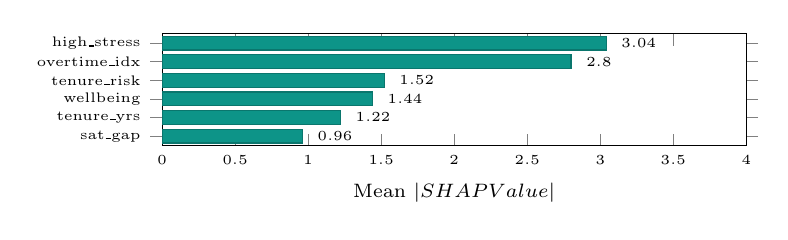
\begin{tikzpicture}
  \begin{axis}[
    xbar, width=9cm, height=3cm,
    xlabel={\scriptsize Mean $|\text{SHAP Value}|$},
    symbolic y coords={sat\_gap, tenure\_yrs, wellbeing, tenure\_risk, overtime\_idx, high\_stress},
    ytick=data,
    xmin=0, xmax=4.0,
    bar width=5pt,
    nodes near coords, nodes near coords align={horizontal},
    every node near coord/.style={font=\tiny, xshift=2pt},
    tick label style={font=\tiny},
    label style={font=\scriptsize},
  ]
  \addplot[fill=teal, draw=teal!80!black] coordinates {
    (0.96,sat\_gap)
    (1.22,tenure\_yrs)
    (1.44,wellbeing)
    (1.52,tenure\_risk)
    (2.80,overtime\_idx)
    (3.04,high\_stress)
  };
  \end{axis}
\end{tikzpicture}
\end{center}

\vspace{-4pt}
\small\textbf{Key:} \texttt{overtime\_index} $\times$ \texttt{wellbeing\_composite} --- combined risk 3$\times$ higher than either alone.
\end{frame}

% ── SLIDE 8: BIAS AUDIT ──────────────────────────────────────
\begin{frame}{6. Bias Audit \& Fairness Metrics}
\small
\textbf{Audited} (not model features): Gender | Age Bracket | Income Bracket\\[4pt]

\footnotesize
\begin{center}
\begin{tabular}{@{}l c c c c c@{}}
  \toprule
  \textbf{Metric} & \textbf{Gender} & \textbf{Age} & \textbf{Income} & \textbf{Thresh.} & \textbf{Pass} \\
  \midrule
  Demogr.\ Parity   & 0.94  & 0.91 & 0.88 & $>0.80$ & \textcolor{green500}{$\cmark$} \\
  TPR Gap            & 0.024 & 0.04 & 0.06 & $<0.10$ & \textcolor{green500}{$\cmark$} \\
  FPR Gap            & 0.02  & 0.03 & 0.05 & $<0.10$ & \textcolor{green500}{$\cmark$} \\
  Disparate Impact   & 0.94  & 0.91 & 0.88 & $>0.80$ & \textcolor{green500}{$\cmark$} \\
  \bottomrule
\end{tabular}
\end{center}

\vspace{4pt}
\small
\textbf{\color{teal}Mitigation Strategies Implemented}
\begin{enumerate}\setlength\itemsep{1pt}\footnotesize
  \item \textbf{Group-specific threshold adjustment} --- equalise TPR across gender
  \item \textbf{Class-weighted re-training} --- \texttt{compute\_sample\_weight('balanced')}
  \item \textbf{Proxy correlation audit} --- flagged $|r| > 0.15$ with sensitive attrs
\end{enumerate}
\end{frame}

% ── SLIDE 9: LIMITATIONS ─────────────────────────────────────
\begin{frame}{7. Limitations \& Future Work}
\footnotesize
\begin{tabular}{@{}p{0.9cm} p{3.4cm} p{0.7cm} p{4cm}@{}}
  \toprule
  \textbf{Cat.} & \textbf{Limitation} & \textbf{Sev.} & \textbf{Mitigation} \\
  \midrule
  Data  & Target leakage: composite from inputs & \textcolor{red500}{High} & Use independent HR outcomes \\[2pt]
  Data  & Synthetic augment.\ (44K $\to$ 500K) & \textcolor{amber}{Med} & Validate on real org data \\[2pt]
  Model & Cross-sectional; no temporal dim. & \textcolor{amber}{Med} & LSTM / Transformer models \\[2pt]
  Fair. & Limited to 3 sensitive attrs & \textcolor{amber}{Med} & Expand; intersectional analysis \\
  \bottomrule
\end{tabular}

\vspace{6pt}
\small
\textbf{\color{teal}Future Work}\\[2pt]
\begin{columns}[T]
\begin{column}{0.46\textwidth}
  \footnotesize
  \textbf{Short-term:} FastAPI + Docker, CI/CD pipeline
\end{column}
\begin{column}{0.46\textwidth}
  \footnotesize
  \textbf{Long-term:} HRIS + MLflow, LSTM + GenAI chatbot
\end{column}
\end{columns}
\end{frame}

% ── SLIDE 10: REPRODUCIBILITY ─────────────────────────────────
\begin{frame}[fragile]{8. Reproducibility \& Deployment}
\small
\begin{columns}[T]
\begin{column}{0.44\textwidth}
  \textbf{\color{teal}GitHub Repository}\\[2pt]
  \scriptsize
\begin{verbatim}
workpulse/
+-- README.md
+-- requirements.txt
+-- Dockerfile
+-- notebooks/
|   +-- 01_problem_framing.ipynb
|   +-- 02_data_collection.ipynb
|   +-- 03_eda_feature_eng.ipynb
|   +-- 04_model_impl.ipynb
|   +-- 05_ethical_ai_bias.ipynb
+-- src/
|   +-- data_pipeline.py
|   +-- train.py
|   +-- predict.py
+-- models/
+-- data/
+-- plots/
\end{verbatim}
\end{column}
\begin{column}{0.52\textwidth}
  \textbf{\color{amber}Saved Artefacts}
  \begin{itemize}\setlength\itemsep{0pt}\footnotesize
    \item 13 model files (joblib \texttt{.pkl})
    \item MLP neural network (\texttt{.keras})
    \item Scaler, PCA, feature column list
    \item RandomizedSearchCV objects
    \item Comparison + CV results CSV
  \end{itemize}

  \vspace{4pt}
  \textbf{\color{amber}Deployment Stack}
  \begin{itemize}\setlength\itemsep{0pt}\footnotesize
    \item \textbf{API:} FastAPI REST endpoint
    \item \textbf{Container:} Docker
    \item \textbf{CI/CD:} Lint + unit tests
    \item \textbf{Tracking:} MLflow / W\&B
    \item \textbf{Versioning:} Rollback plan
  \end{itemize}
\end{column}
\end{columns}
\end{frame}

% ── SLIDE 11: SUMMARY ────────────────────────────────────────
{
\setbeamercolor{background canvas}{bg=slate900}
\setbeamercolor{normal text}{fg=white}
\usebeamercolor[fg]{normal text}
\begin{frame}{Summary}

\begin{itemize}\setlength\itemsep{8pt}
  \item[\textcolor{teal}{$\cmark$}] \textbf{11 models} across 5 phases $\rightarrow$ \textbf{XGBoost selected} (F1=0.91, AUC=0.99)
  \item[\textcolor{teal}{$\cmark$}] \textbf{4 explainability tools}: SHAP, LIME, PDP, ICE --- full coverage
  \item[\textcolor{teal}{$\cmark$}] \textbf{Fairness audit}: all metrics pass across gender, age, income
  \item[\textcolor{teal}{$\cmark$}] \textbf{8 limitations} documented with severity and mitigation plans
  \item[\textcolor{teal}{$\cmark$}] \textbf{End-to-end reproducible}: models, configs, Docker ready
\end{itemize}

\vspace{16pt}
\begin{center}
  {\Large\color{teal} Questions \& Discussion}\\[6pt]
  {\color{slate400}\textit{WorkPulse: Predicting burnout before it costs you your best people.}}
\end{center}

\end{frame}
}

\end{document}
